% !TeX root = ../paper.tex

\appendix
\section{ITrace 补充分析}

\begin{figure}[H]
  \centering
  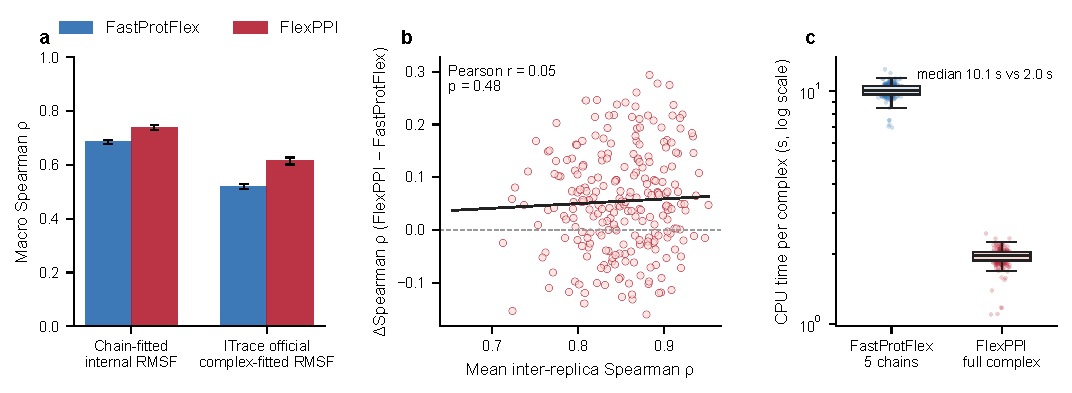
\includegraphics[width=\textwidth]{fig_itrace_sensitivity.pdf}
  \caption{ITrace 标签定义与样本纳入规则的敏感性分析。主分析使用逐链拟合的
  $C_\alpha$ RMSF，并排除唯一精确训练 PDB 重叠 3KXF；次分析改用 ITrace
  官方全复合体拟合标签，或把 3KXF 加回全部 245 个复合体。逐链拟合标签减少
  链间整体运动对链内柔性的污染；两种纳入规则下总体排序不变，而官方标签下
  FlexPPI 相对 FastProtFlex 的优势更大，说明主要结论并非由单一样本或单一
  对齐定义造成。误差线为 2,000 次复合体 bootstrap 95\% 置信区间。}
  \label{fig:itrace-sensitivity}
\end{figure}

\subsection{轨迹覆盖、预测成功率与标签质量控制}

本研究使用的 ITrace 数据快照包含 245 个复合体和 735 条轨迹，即每个复合体三条独立重复。
每条轨迹实际保留 1,001--1,009 帧，标签计算使用全部可用帧；FastProtFlex 的
1,225 个逐链预测和 FlexPPI 的 245 个整复合体预测均成功完成。主标签共同覆盖
200,501/200,501 个可比较残基，官方全复合体拟合标签覆盖
200,430/200,501 个残基，即 99.965\%。244 个精确 PDB 外部复合体的重复间
平均 Spearman 均不低于 0.5，中位数为 0.853；模型优势与重复可靠性的 Pearson
相关仅为 0.05（$p=0.48$），未观察到 FlexPPI 的改善只集中在低可靠标签上的
迹象。

\subsection{长度外推与运行时间}

ITrace 复合体长度为 599--848 个残基，中位数为 826；其中 235/245 超过预训练
配置中的 768 残基上限。当前推理程序没有截断输入，因此所有残基均参与预测，
但这仍属于训练长度范围之外的外推，应在后续长度分层和更长复合体训练中单独
验证。在同一批 CPU 运行记录中，FastProtFlex 完成五条链的中位时间为
10.1 秒，FlexPPI 完成整个复合体的中位时间为 2.0 秒，约快 5.1 倍；该时间只
反映当前硬件、批处理和实现，不作为算法复杂度的普适结论。

\subsection{冻结检查点上下文消融的完整性控制}

上下文消融复用正文完整复合体预测，只额外运行同一检查点的结合态孤立链
前向推理。检查点 SHA256 与完整复合体评估逐字节一致；推理函数在
\texttt{torch.no\_grad()} 下运行，未构建优化器，也未读取 ITrace RMSF
标签来调整模型参数、阈值或模拟条件。245 个复合体共生成 1,225 个单链输入，
全部推理成功，中位耗时为 0.199\,s/链，总耗时为 240.5\,s。孤立链预测与主
标签在 200,501 个共同残基上一一匹配，无缺失或重复键；排除 3KXF 后，
正文分析包含 244 个复合体、1,220 条链和 199,668 个残基。

孤立链由同一结合态拓扑直接删除其他链的 \texttt{ATOM} 记录得到，目标链
坐标不作能量最小化、结构预测或重新对齐。这一设计最大程度保持目标链自身
几何不变，但仍同时改变了跨链接触、输入总长度和全局注意力归一化。尤其是
完整 ITrace 输入中有 235/245 个复合体超过预训练配置的 768 残基上限，而
孤立链通常回到训练长度范围，约 9--15 残基的孤立抗原肽又位于另一个极端。
因此，正文把完整减孤立称为“上下文响应”，不把它解释为真实 apo/holo
$\Delta$RMSF 或纯粹的跨链边贡献。

\subsection{正文分层结果的完整数值}

表 \ref{tab:itrace-overall} 给出完整复合体 FlexPPI 与逐链 FastProtFlex 的全部
共同指标，表 \ref{tab:itrace-context-ablation} 给出同一 FlexPPI 检查点的
完整复合体/孤立链消融。表 \ref{tab:itrace-context-sensitivity} 报告排除短
抗原肽后的结果，表 \ref{tab:itrace-regions} 报告区域分层结果。

% !TeX root = ../paper.tex

\begin{table}[H]
  \centering
  \caption{完整复合体 FlexPPI 与逐链 FastProtFlex 在 244 个 ITrace
  复合体上的等权平均结果。}
  \label{tab:itrace-overall}
  \small
  \resizebox{\textwidth}{!}{%
  \begin{tabular}{lrrrrrrr}
    \toprule
    方法 &
    Spearman $\uparrow$ & Pearson $\uparrow$ &
    z-MAE $\downarrow$ & z-RMSE $\downarrow$ &
    AUROC $\uparrow$ & AP $\uparrow$ & P@K $\uparrow$ \\
    \midrule
    FastProtFlex
      & 0.685 & 0.619 & 0.626 & 0.828 & 0.841 & 0.678 & 0.581 \\
    FlexPPI
      & \textbf{0.740} & \textbf{0.677} &
        \textbf{0.531} & \textbf{0.753} &
        \textbf{0.871} & \textbf{0.735} & \textbf{0.631} \\
    \bottomrule
  \end{tabular}%
  }
\end{table}


% !TeX root = ../paper.tex

\begin{table}[H]
  \centering
  \caption{同一冻结 FlexPPI 检查点的完整复合体与孤立链输入比较。
  ``完整输入优势'' 对误差指标取反，因此正值均表示完整输入更优。}
  \label{tab:itrace-context-ablation}
  \small
  \resizebox{\textwidth}{!}{%
  \begin{tabular}{lrrrrl}
    \toprule
    指标 &
    完整复合体 &
    孤立链 &
    完整输入优势 &
    95\% CI &
    双侧 Wilcoxon $p$ \\
    \midrule
    Spearman $\uparrow$
      & 0.740 & 0.683 & 0.057 & $[0.045,0.069]$ & $1.47\times10^{-15}$ \\
    Pearson $\uparrow$
      & 0.677 & 0.621 & 0.057 & $[0.044,0.069]$ & $1.10\times10^{-14}$ \\
    z-MAE $\downarrow$
      & 0.531 & 0.571 & 0.040 & $[0.030,0.049]$ & $2.46\times10^{-14}$ \\
    z-RMSE $\downarrow$
      & 0.753 & 0.813 & 0.060 & $[0.048,0.071]$ & $2.31\times10^{-19}$ \\
    Top-20\% AUROC $\uparrow$
      & 0.871 & 0.836 & 0.035 & $[0.026,0.044]$ & $9.33\times10^{-13}$ \\
    Top-20\% AP $\uparrow$
      & 0.735 & 0.658 & 0.077 & $[0.068,0.085]$ & $5.42\times10^{-33}$ \\
    Top-20\% P@K $\uparrow$
      & 0.631 & 0.576 & 0.056 & $[0.045,0.066]$ & $1.08\times10^{-18}$ \\
    绝对 MAE（\AA）$\downarrow$
      & 0.346 & 1.865 & 1.519 & $[1.506,1.531]$ & $8.89\times10^{-42}$ \\
    绝对 RMSE（\AA）$\downarrow$
      & 0.475 & 1.998 & 1.523 & $[1.510,1.535]$ & $8.89\times10^{-42}$ \\
    \bottomrule
  \end{tabular}%
  }
\end{table}


% !TeX root = ../paper.tex

\begin{table}[H]
  \centering
  \caption{短肽排除敏感性分析。Spearman 优势为完整减孤立；绝对 MAE
  优势为孤立减完整，故两列中的正优势均表示完整复合体输入更优。
  ``非肽链'' 对每个复合体的 MHC、$\beta_2$m、TCR$\alpha$ 和
  TCR$\beta$ 四条链等权平均。}
  \label{tab:itrace-context-sensitivity}
  \small
  \resizebox{\textwidth}{!}{%
  \begin{tabular}{llrrrrl}
    \toprule
    队列 & 指标 &
    完整复合体 &
    孤立链 &
    完整输入优势 &
    95\% CI &
    双侧 Wilcoxon $p$ \\
    \midrule
    全部五链
      & Spearman
      & 0.740 & 0.683 & 0.057 & $[0.045,0.069]$ & $1.47\times10^{-15}$ \\
    全部五链
      & 绝对 MAE（\AA）
      & 0.346 & 1.865 & 1.519 & $[1.506,1.531]$ & $8.89\times10^{-42}$ \\
    非肽链
      & Spearman
      & 0.849 & 0.830 & 0.019 & $[0.017,0.022]$ & $1.11\times10^{-27}$ \\
    非肽链
      & 绝对 MAE（\AA）
      & 0.376 & 0.348 & $-0.028$ & $[-0.031,-0.025]$ & $3.21\times10^{-33}$ \\
    \bottomrule
  \end{tabular}%
  }
\end{table}


% !TeX root = ../paper.tex

\begin{table}[H]
  \centering
  \caption{ITrace 外部队列上的区域分层性能。$\Delta$ 定义为
  FlexPPI 减 FastProtFlex；正值有利于 FlexPPI。加粗差异通过按指标跨区域
  的 Benjamini--Hochberg 校正（$q<0.05$）。}
  \label{tab:itrace-regions}
  \scriptsize
  \resizebox{\textwidth}{!}{%
  \begin{tabular}{lrrrrrrrr}
    \toprule
    区域 &
    Fast $\rho$ & Flex $\rho$ & $\Delta\rho$ & FDR $q$ &
    Fast AP & Flex AP & $\Delta$AP & FDR $q$ \\
    \midrule
    总体
      & 0.685 & 0.740 & \textbf{0.054} & $2.6{\times}10^{-13}$
      & 0.678 & 0.735 & \textbf{0.057} & $2.1{\times}10^{-23}$ \\
    TCR--pMHC 界面
      & 0.481 & 0.454 & -0.027 & 0.055
      & 0.663 & 0.667 & 0.003 & 0.92 \\
    非界面
      & 0.760 & 0.810 & \textbf{0.049} & $5.8{\times}10^{-18}$
      & 0.728 & 0.780 & \textbf{0.051} & $2.1{\times}10^{-23}$ \\
    pMHC
      & 0.610 & 0.663 & \textbf{0.053} & $1.3{\times}10^{-5}$
      & 0.650 & 0.682 & \textbf{0.033} & $1.4{\times}10^{-5}$ \\
    TCR
      & 0.798 & 0.855 & \textbf{0.056} & $1.8{\times}10^{-36}$
      & 0.721 & 0.815 & \textbf{0.094} & $2.3{\times}10^{-38}$ \\
    抗原肽
      & 0.119 & 0.302 & \textbf{0.183} & $4.5{\times}10^{-7}$
      & 0.444 & 0.571 & \textbf{0.127} & $3.8{\times}10^{-8}$ \\
    CDR1
      & 0.858 & 0.867 & 0.009 & 0.16
      & 0.811 & 0.799 & -0.013 & 0.30 \\
    CDR2
      & 0.833 & 0.849 & 0.016 & 0.055
      & 0.812 & 0.834 & \textbf{0.022} & 0.021 \\
    CDR3
      & 0.894 & 0.812 & \textbf{-0.082} & $8.2{\times}10^{-26}$
      & 0.805 & 0.729 & \textbf{-0.075} & $1.7{\times}10^{-11}$ \\
    TCR framework
      & 0.801 & 0.875 & \textbf{0.074} & $7.4{\times}10^{-38}$
      & 0.752 & 0.838 & \textbf{0.086} & $2.3{\times}10^{-38}$ \\
    \bottomrule
  \end{tabular}%
  }
\end{table}


\subsection{可审计数据产物}

正文表格和图的精简数值源随论文保存在
{\footnotesize\path{data/itrace/summary_metrics.csv}}、
{\footnotesize\path{data/itrace/paired_tests.csv}}、
{\footnotesize\path{data/itrace/table_overall.csv}}、
{\footnotesize\path{data/itrace/table_regions.csv}} 和
{\footnotesize\path{data/itrace/cdr3_diagnostic_per_complex.csv}}。完整逐残基预测、
逐复合体指标、bootstrap 抽样结果及运行日志保留在项目的
{\footnotesize\path{output/itrace_benchmark/}} 中；论文只复制生成图表和核验结论所需的
精简原始表，避免把模型缓存或中间二进制文件误当成实验数据。

上下文消融的图形源数据另存于
{\footnotesize\path{data/itrace_context/}}，包括 244 个复合体的配对
Spearman、七项指标优势、五类链的分层结果和完整的 3,660 条
“复合体--链角色--输入条件”RMSF 尺度记录。生成脚本为
{\footnotesize\path{figures/make_itrace_context_ablation_figure.py}}，
完整统计与数据来源记录为
{\footnotesize\path{figures/fig_itrace_context_ablation_statistics.json}}；
未经精简的逐残基预测和推理日志保留在
{\footnotesize\path{output/itrace_zero_shot_context/}}。
